\documentclass[12pt]{article}
%%%%%%%%%%%%%%%%%%%%%%%%%%%%%
% Préambulo
%
\usepackage[T1]{fontenc}
\usepackage[utf8]{inputenc}
\usepackage[spanish,es-tabla]{babel}% agregamos es-tabla para que la descripcion de las tablas comiencen con TABLA%
\parindent=0cm %modificar tamaño de sangria 
\usepackage{amsmath}
\usepackage{amssymb,amsfonts,latexsym,cancel}
\usepackage{graphicx}
\usepackage{epstopdf}
\usepackage{float}
\usepackage{subfigure}
%
\usepackage{array} %Para usar el comando m{Ancho}%
\newcolumntype{E}{>{$}c<{$}} %Definiendo un nuevo comando, La E puede ser cualquier letra, el segundo es el tipo de columna. Para usar colocamos la letra E%
\usepackage{longtable}
%%%%%%%%%%%%%%%%%%%%%%%%%%%%
\begin{document}
\title{Práctica 5. \\ Tablas}
\author{Edison Achalma}
\date{}
\maketitle
\tableofcontents

\section{Incluir tablas básicas}
En \LaTeX  \, la forma básica en la que podemos incluir tablas es usando el entorno \textbf{tabular}, su sintaxis es la siguiente.\\[0.3cm]
\noindent \textbf{Formato de las columnas:}
\begin{itemize}
\item l (alineado a la izquierda)
\item c (alineado a la centrada)
\item r (alineado a la derecha)
\end{itemize}

\begin{itemize}
\item $ \& $ carácter que se utiliza para separar columnas
\end{itemize}

Nuestra primera tabla \quad
\begin{tabular}{lcr} % Este configuración {lcr} indica que los datos de la primara columna van a la izquierda, la segunda columna centrada y los de la tercera columna van a la derecha%
Lunes & Martes & Miércoles  \\
0     &      0 & 0 \\
1     &      1 & 1
\end{tabular}

\newpage

\subsection{Entorno table -tablas con líneas-}

\begin{table}[!ht]
\centering %centrara tabla%
\begin{tabular}{ll}
t & coloca la tabla en a parte superior (top)\\
b & coloca la tabla en la parte inferior (bottom) \\
h & coloca la tabla donde le indiquemos (here)
%cada columna separada con un & y las filas con doble barra \\ %
\end{tabular}
\caption{Descripción del entorno tabla}
\label{Tabla1}
\end{table}

\begin{table}[H]
\centering
\begin{tabular}{lc}
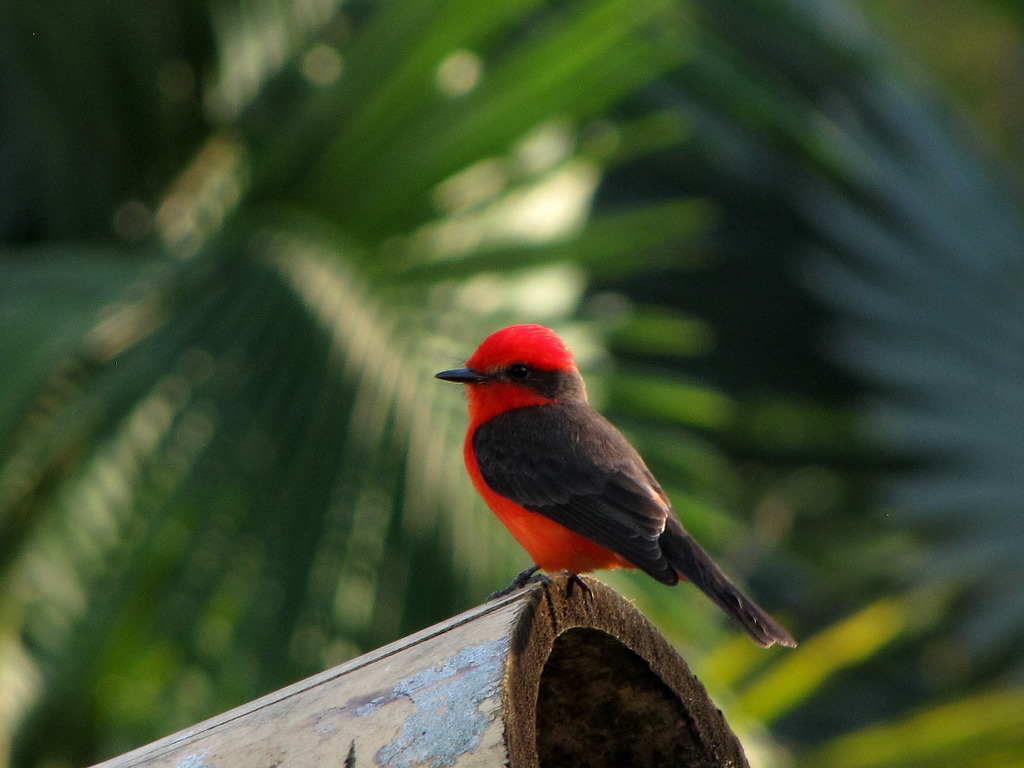
\includegraphics[scale=0.1]{figuras/Petirrojo2} & imagen 1 \\
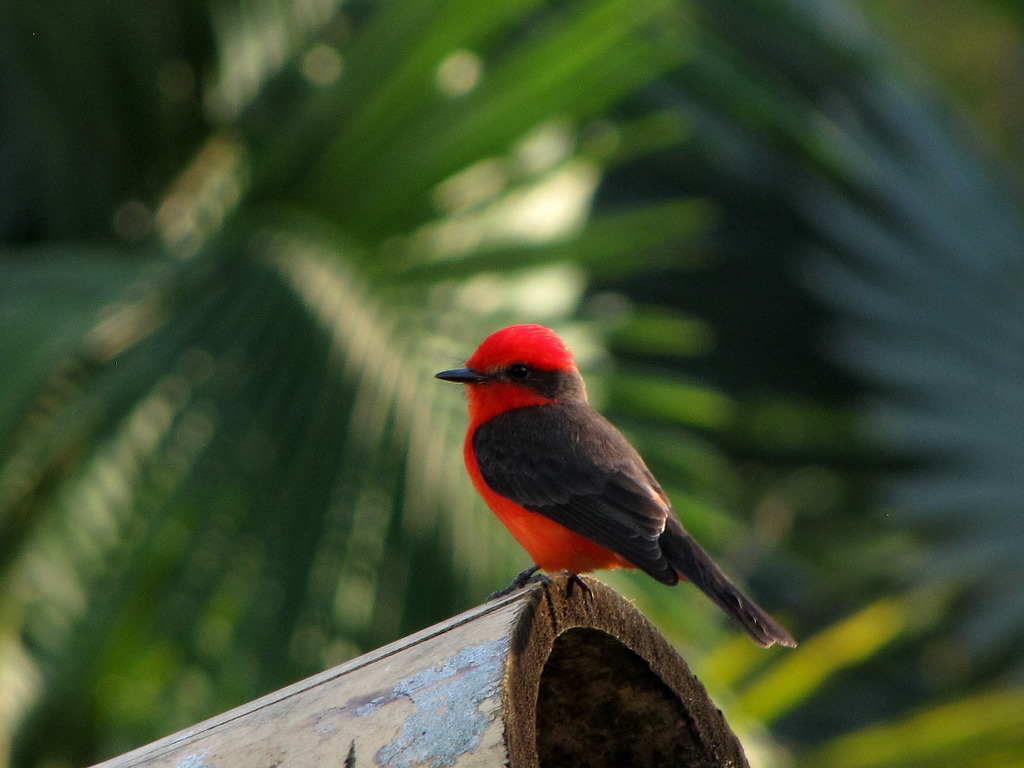
\includegraphics[scale=0.1]{figuras/Petirrojo2} & imagen 2 \\
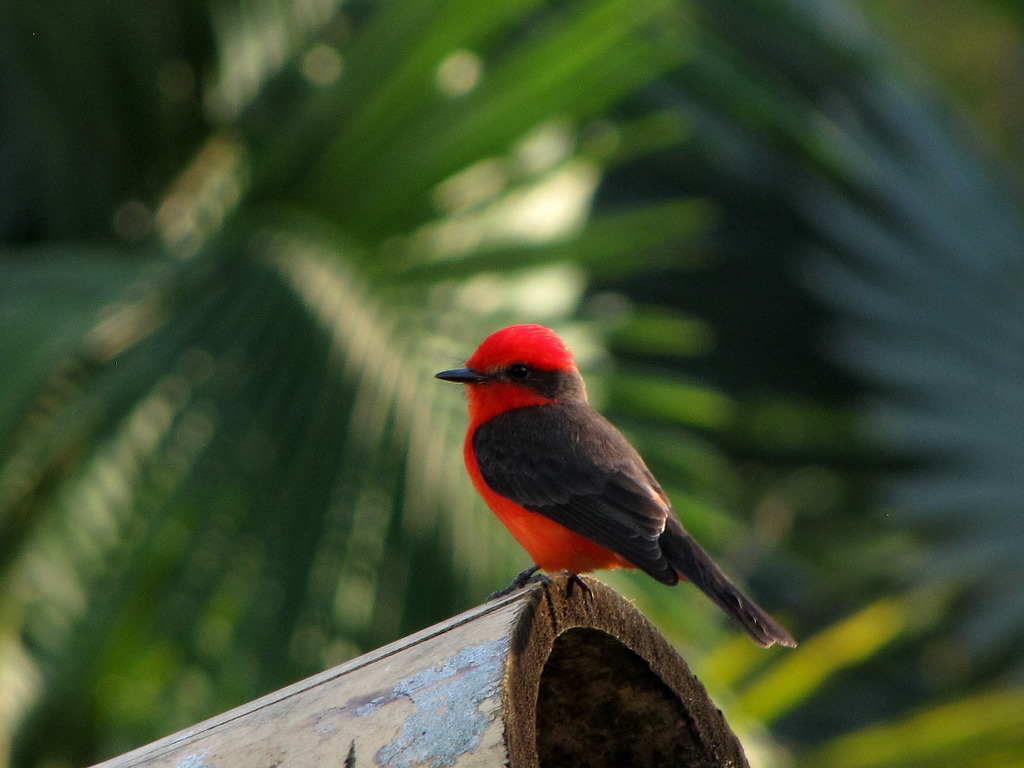
\includegraphics[scale=0.1]{figuras/Petirrojo2} & imagen 3 
\end{tabular}
\caption{Incluir imágenes}
\label{incluirimagen}
\end{table}

\begin{table}[H]
\centering
\begin{tabular}{||l|c|}
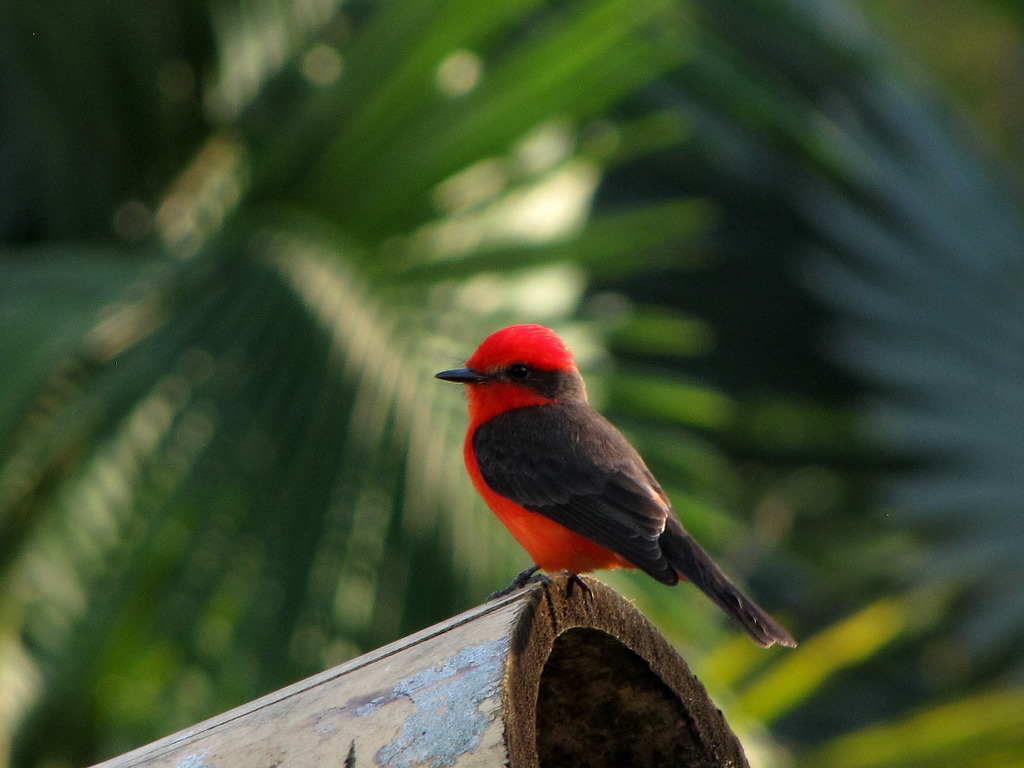
\includegraphics[scale=0.1]{figuras/Petirrojo2} & imagen 1 \\
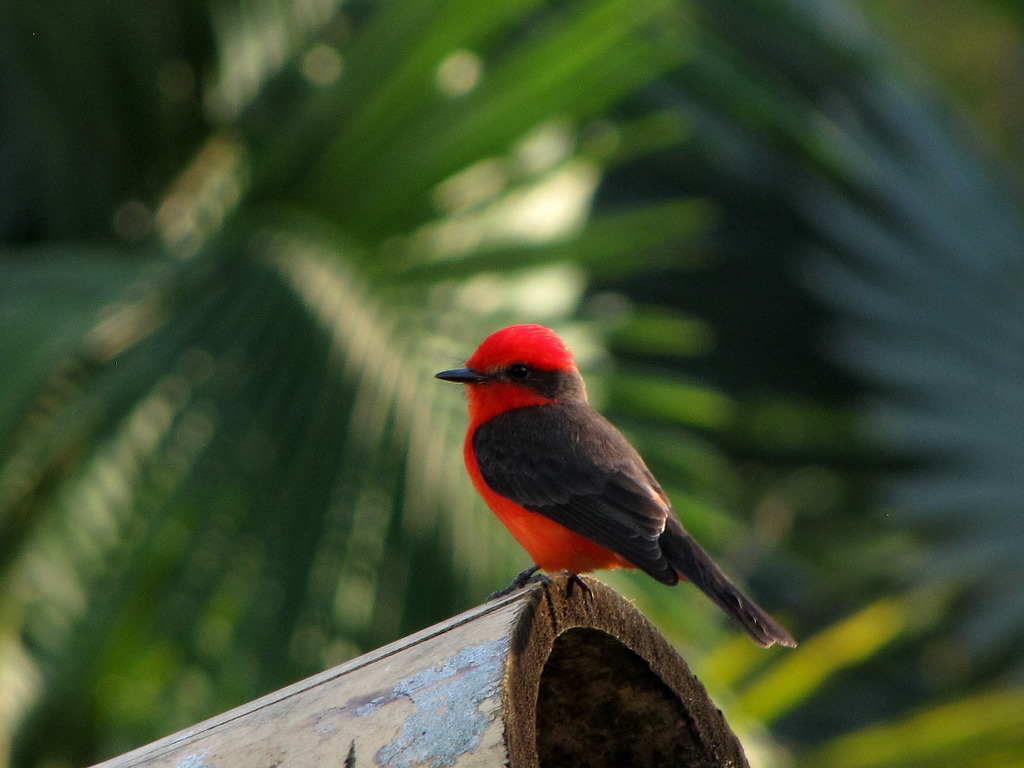
\includegraphics[scale=0.1]{figuras/Petirrojo2} & imagen 2 \\
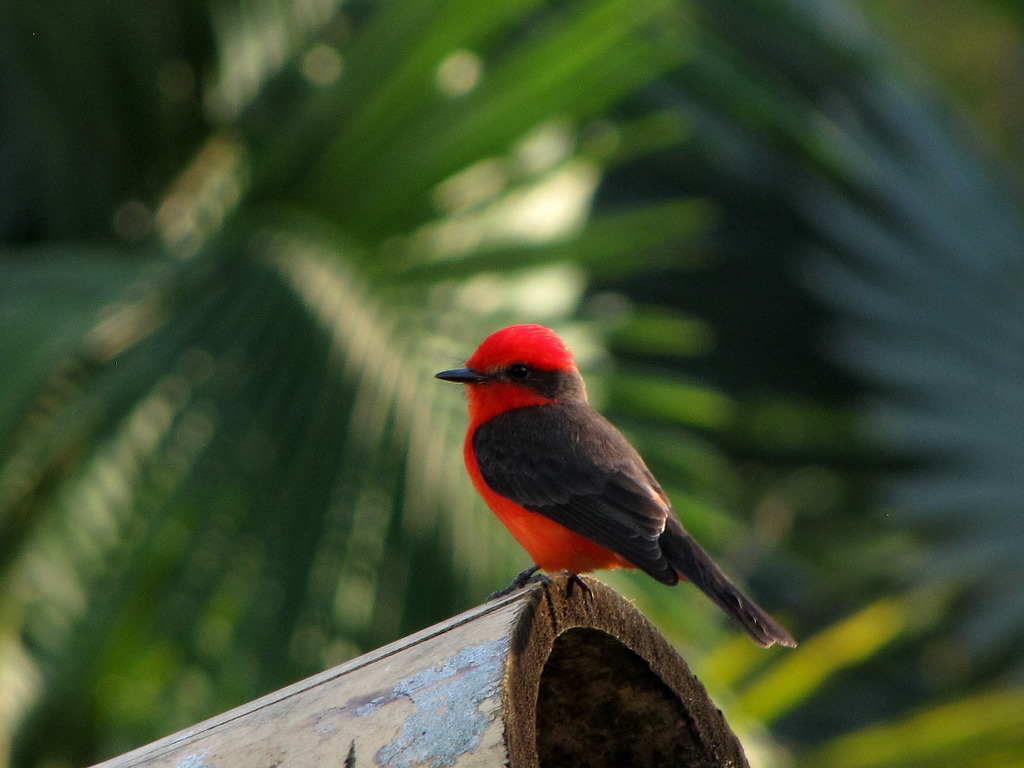
\includegraphics[scale=0.1]{figuras/Petirrojo2} & imagen 3 
\end{tabular}
\caption{Incluir imágenes separas con líneas}
\label{incluirimagen}
\end{table}

\begin{table}[H]
\centering
\begin{tabular}{|l|c|r|}
\hline
Lunes & Martes & Miércoles \\
\hline %líneas horizontales%
0     &      0 & 0 \\
1     &      1 & 1 \\
\hline
\end{tabular}
\caption{Tabla con líneas}
\label{incluirimagen1}
\end{table}

\begin{table}[H]
\centering
\begin{tabular}{|l|c|r|c|}
\hline
Lunes & Martes & Miércoles & Jueves\\
\hline %líneas horizontales%
0     &      0 & 0         & 0\\
\cline{1-2} %La línea solamente abarca la comulna 1 y 2%
1     &      1 & 1         & 0\\
\cline{1-3}
1     &      1 & 1         & 0\\
\hline
\end{tabular}
\caption{Tabla con líneas de diferentes tamaños}
\label{incluirimagen1}
\end{table}

\newpage
Ejemplo de tablas con líneas

\begin{table}[H]
\centering
\begin{tabular}{|l|c|r|c|}
\hline
Lunes & Martes & Miércoles & Jueves\\
\hline %líneas horizontales%
0     &      0 & 0         & 0\\
\cline{2-4} %La línea abarca la comulna 2 a 4%
1     &      1 & 1         & 0\\
\cline{3-4}
1     &      1 & 1         & 0\\
\hline
\end{tabular}
\caption{Tabla con líneas de diferentes tamaños}
\label{incluirimagen1}
\end{table}

\subsection{Múltiples columnas}

\begin{table}[H]
\centering
\begin{tabular}{|l|c|r|c|}
\hline
\multicolumn{2}{|c|}{Enero} & & \\ %El comando multicolumn hace que las letras vayan en varias columnas por ejemplo la {2} indica que solo abarque dos columnas, {|c|} las letra van centradas entre líneas verticales y {Enero} son las teras en mención, finalmente & &  estos dos símbolos sirven para completar las columnas no afectadas%
\hline
\multicolumn{4}{|c|}{Días de la semana} \\
\hline
Lunes & Martes & Miércoles & Jueves\\
\hline %líneas horizontales%
0     &      0 & 0         & 0\\
\cline{2-4} %La línea abarca la comulna 2 a 4%
1     &      1 & 1         & 0\\
\cline{3-4}
1     &      1 & 1         & 0\\
\hline
\end{tabular}
\caption{Tabla con líneas de diferentes tamaños}
\label{incluirimagen1}
\end{table}

\begin{table}[H]
\centering
\begin{tabular}{|l|c|r|c|}
\hline
\multicolumn{2}{|c|}{Enero} & & \\ 
\hline
& \multicolumn{3}{|c|}{Días de la semana 2} \\
\hline
Lunes & Martes & Miércoles & Jueves\\
\hline %líneas horizontales%
0     &      0 & 0         & 0\\
\cline{2-4} %La línea abarca la comulna 2 a 4%
1     &      1 & 1         & 0\\
\cline{3-4}
1     &      1 & 1         & 0\\
\hline
\end{tabular}
\caption{Tabla con líneas de diferentes tamaños}
\label{incluirimagen1}
\end{table}

\subsection{Tablas con párrafos}

\begin{table}[H]
\centering
\begin{tabular}{|l|p{6cm}|} %La segunda columna es de 6cm%
\hline
Comando & Descripción \\
\hline
p$\{$Ancho$\}$ & Crea una columna con un ancho fijo. El contenido de esta celda se compone de un párrafo ordinario, sin sangría inicial \\
\hline
m$\{$Ancho$\}$ & Crea una columna con un ancho fijo. El párrafo aparece verticalmente centrado respecto a las columnas vecinas \\ 
\hline
\end{tabular}
\caption{Tabla con párrafos}
\label{tablaconpárrafo}
\end{table}

\begin{table}[H]
\centering
\begin{tabular}{|l|m{6cm}|} %La segunda columna es de 6cm%
\hline
Comando & Descripción \\
\hline
p$\{$Ancho$\}$ & Crea una columna con un ancho fijo. El contenido de esta celda se compone de un párrafo ordinario, sin sangría inicial \\
\hline
m$\{$Ancho$\}$ & Crea una columna con un ancho fijo. El párrafo aparece verticalmente centrado respecto a las columnas vecinas \\ 
\hline
\end{tabular}
\caption{Tabla con párrafos}
\label{tablaconpárrafo}
\end{table}

\subsection{Escalar una tabla}

\begin{table}[H]
\centering
\scalebox{0.8}{
\begin{tabular}{|l|m{6cm}|} %La segunda columna es de 6cm%
\hline
Comando & Descripción \\
\hline
p$\{$Ancho$\}$ & Crea una columna con un ancho fijo. El contenido de esta celda se compone de un párrafo ordinario, sin sangría inicial \\
\hline
m$\{$Ancho$\}$ & Crea una columna con un ancho fijo. El párrafo aparece verticalmente centrado respecto a las columnas vecinas \\ 
\hline
\end{tabular}
}
\caption{Tabla con escala 0.8}
\label{tablaconpárrafo}
\end{table}

\section{Expresiones, símbolos matemáticos en tablas}

\begin{table}[H]
\centering
\begin{tabular}{|l|c|c|}
\hline
Matemática & $x+1$ & $\lambda$ \\
\hline
Ejemplo & $x_{2}$ & $x_{3}$ \\
\hline
$(a+b)^{2}$ & $(a+b)^{3}$ & $(a+b)^{4}$ \\
\hline
\end{tabular}
\caption{Usar expresiones matemáticas de forma manual}
\end{table}

\begin{table}[H]
\centering
\begin{tabular}{|>{$}c<{$}|>{$}c<{$}|>{$}c<{$}|} %Aquí hay tres columnas que indican que las letras serán centradas y entre $$%
\hline
Ejemplo 1 & x+1 & \lambda \\
\hline
\text{Ejemplo 1} & x_{2} & x_{3} \\ %comando para insertar texto%
\hline
(a+b)^{2} & (a+b)^{3} & (a+b)^{4} \\
\hline
\end{tabular}
\caption{Usar expresiones matemáticas de forma automática, sin usar los el símbolo dólar}
\end{table}

\begin{table}[H]
\centering
\begin{tabular}{|E|E|E|} 
\hline
Ejemplo 1 & x+1 & \lambda \\
\hline
\text{Ejemplo 1} & x_{2} & x_{3} \\ %comando para insertar texto%
\hline
(a+b)^{2} & (a+b)^{3} & (a+b)^{4} \\
\hline
\end{tabular}
\caption{Usar expresiones matemáticas con el nuevo comando definido E}
\end{table}

\section{Tablas largas, paquete longtable}

\begin{longtable}[C]{|ccc|}
Nombre & Teléfono & Edad \\
Nombre & Teléfono & Edad \\
Nombre & Teléfono & Edad \\
Nombre & Teléfono & Edad \\
Nombre & Teléfono & Edad \\
Nombre & Teléfono & Edad \\
Nombre & Teléfono & Edad \\
Nombre & Teléfono & Edad \\
Nombre & Teléfono & Edad \\
Nombre & Teléfono & Edad \\
A & 12345 & 20 \\
Nombre & Teléfono & Edad \\
Nombre & Teléfono & Edad \\
Nombre & Teléfono & Edad \\
Nombre & Teléfono & Edad \\
Nombre & Teléfono & Edad \\
Nombre & Teléfono & Edad \\
Nombre & Teléfono & Edad \\
Nombre & Teléfono & Edad \\
Nombre & Teléfono & Edad \\
Nombre & Teléfono & Edad \\
A & 12345 & 20 \\
Nombre & Teléfono & Edad \\
Nombre & Teléfono & Edad \\
Nombre & Teléfono & Edad \\
Nombre & Teléfono & Edad \\
Nombre & Teléfono & Edad \\
Nombre & Teléfono & Edad \\
Nombre & Teléfono & Edad \\
Nombre & Teléfono & Edad \\
Nombre & Teléfono & Edad \\
Nombre & Teléfono & Edad \\
A & 12345 & 20 \\
Nombre & Teléfono & Edad \\
Nombre & Teléfono & Edad \\
Nombre & Teléfono & Edad \\
Nombre & Teléfono & Edad \\
Nombre & Teléfono & Edad \\
Nombre & Teléfono & Edad \\
Nombre & Teléfono & Edad \\
Nombre & Teléfono & Edad \\
Nombre & Teléfono & Edad \\
Nombre & Teléfono & Edad \\
A & 12345 & 20 \\
\caption{Tabla larga}
\label{TablaLargaEjemplo}
\end{longtable}



\end{document}